% Compile with: pdflatex (run TWICE to resolve cross-references)
% Place in writeups/ alongside the paper; figures are in ../output/
\documentclass[10pt,aspectratio=169]{beamer}

% ── Theme ────────────────────────────────────────────────────────────────────
\usetheme{Madrid}
\usecolortheme{default}

% MIT crimson (#A31F34) as primary structure color
\definecolor{mitcrimson}{HTML}{A31F34}
\definecolor{mitgray}{HTML}{8A8B8C}
\definecolor{mitwarm}{HTML}{F2F2F0}

\setbeamercolor{structure}{fg=mitcrimson}
\setbeamercolor{palette primary}{bg=mitcrimson, fg=white}
\setbeamercolor{palette secondary}{bg=mitcrimson!80, fg=white}
\setbeamercolor{palette tertiary}{bg=mitcrimson!60, fg=white}
\setbeamercolor{palette quaternary}{bg=mitcrimson, fg=white}
\setbeamercolor{frametitle}{bg=mitcrimson, fg=white}
\setbeamercolor{title}{fg=white}
\setbeamercolor{subtitle}{fg=white!85}
\setbeamercolor{author in head/foot}{bg=mitcrimson!80}
\setbeamercolor{title in head/foot}{bg=mitcrimson}
\setbeamercolor{date in head/foot}{bg=mitcrimson!60}
\setbeamercolor{block title}{bg=mitcrimson!15, fg=mitcrimson}
\setbeamercolor{block body}{bg=mitwarm}
\setbeamercolor{alerted text}{fg=mitcrimson}

% ── Packages ──────────────────────────────────────────────────────────────────
\usepackage[T1]{fontenc}
\usepackage[utf8]{inputenc}
\usepackage{lmodern}
\usepackage{amsmath,amssymb}
\usepackage{graphicx}
\usepackage{booktabs}
\usepackage{microtype}

% ── Beamer settings ───────────────────────────────────────────────────────────
\setbeamertemplate{navigation symbols}{}          % remove nav bar
\setbeamertemplate{footline}{%
  \leavevmode%
  \hbox{%
    \begin{beamercolorbox}[wd=.333\paperwidth,ht=2.25ex,dp=1ex,center]{author in head/foot}%
      \usebeamerfont{author in head/foot}\insertshortauthor
    \end{beamercolorbox}%
    \begin{beamercolorbox}[wd=.334\paperwidth,ht=2.25ex,dp=1ex,center]{title in head/foot}%
      \usebeamerfont{title in head/foot}\insertshorttitle
    \end{beamercolorbox}%
    \begin{beamercolorbox}[wd=.333\paperwidth,ht=2.25ex,dp=1ex,right]{date in head/foot}%
      \usebeamerfont{date in head/foot}\insertshortdate\hspace*{2em}%
      \insertframenumber{}/\inserttotalframenumber\hspace*{1.5ex}
    \end{beamercolorbox}%
  }\vskip0pt%
}
\setbeamertemplate{itemize items}[circle]
\setbeamersize{text margin left=0.9em, text margin right=0.9em}
\setbeamerfont{frametitle}{size=\large, series=\bfseries}
\setbeamerfont{block title}{size=\normalsize, series=\bfseries}

% Inline citations used throughout (no .bib file needed for presentation)

% ─────────────────────────────────────────────────────────────────────────────
\title[EGS Giveaways \& Steam Engagement]{%
  Epic Games Store Giveaways:\\[0.2em]
  Causal Effect on Steam Player Engagement}
\subtitle{14.33 Research Paper --- Final Presentation}
\author[Nicholas Liu]{Nicholas Liu}
\institute{MIT Department of Economics}
\date{Spring 2026}

% ═════════════════════════════════════════════════════════════════════════════
\begin{document}

% ── TITLE SLIDE ──────────────────────────────────────────────────────────────
\begin{frame}
  \titlepage
\end{frame}

% ── SLIDE 1: MOTIVATION & RESEARCH QUESTION ──────────────────────────────────
\begin{frame}{Motivation \& Research Question}

\begin{columns}[T]
\column{0.56\textwidth}
  \textbf{The puzzle}
  \begin{itemize}
    \item Epic Games Store (EGS) has given away \alert{541 games for free} since 2018 --- its primary differentiation lever against Steam
    \item Standard theory predicts a \alert{zero-price substitute} on a rival platform diverts players \emph{away} from Steam
    \item But in January 2026, New Blood CEO Dave Oshry reported that giving away \textit{Blood West} on EGS caused Steam sales to surge \alert{$\sim$200\%} the same day
  \end{itemize}

  \vspace{0.7em}
  \textbf{Research question}
  \begin{block}{}
    Does an EGS free giveaway \emph{increase} or \emph{decrease} Steam player engagement for the same game --- and how does this evolve over time?
  \end{block}

\column{0.42\textwidth}
  \textbf{Two competing mechanisms}
  \vspace{0.4em}

  \textbf{Advertising:} Giveaway generates media buzz $\rightarrow$ players flock to Steam (primary discovery/community layer) $\rightarrow$ \alert{positive} short-run spillover

  \vspace{0.6em}
  \textbf{Substitution:} Free copy on Epic gradually diverts playtime away from Steam $\rightarrow$ \alert{negative} medium-run effect

  \vspace{0.6em}
  \textit{Both may operate, but at different horizons.}
\end{columns}

\end{frame}

% ── SLIDE 2: DATA ────────────────────────────────────────────────────────────
\begin{frame}{Data}

\begin{columns}[T]
\column{0.48\textwidth}
  \textbf{EGS Giveaway History}
  \begin{itemize}
    \item Kaggle dataset (Dongre, 2025): every free game on EGS Dec 2018--2025
    \item 541 events $\rightarrow$ \alert{471 unique titles}; 70 repeat appearances
    \item 63 titles given away more than once (30 within 12 months = ``proximate'')
  \end{itemize}

  \vspace{0.5em}
  \textbf{Steam Player Data}
  \begin{itemize}
    \item Monthly average concurrent players scraped from SteamCharts for each matched game
    \item Panel: July 2012 -- February 2026
    \item Outcome: $\ln(\texttt{avg\_players} + 1)$
  \end{itemize}

\column{0.50\textwidth}
  \textbf{Final Panel}

  \vspace{0.3em}
  \begin{tabular}{lc}
    \toprule
    & \\[-0.8em]
    Games in final panel & \alert{446} \\
    Game-month observations & \alert{38,642} \\
    Median game: months of data & 88 \\
    \midrule
    Mean avg.\ players/month & 1,584 \\
    \quad (median) & 65 \\
    Mean $\ln(\texttt{avg\_players}+1)$ & 4.43 \\
    \bottomrule
  \end{tabular}

  \vspace{0.6em}
  \textit{\small Player counts are heavily right-skewed --- 101 games have pre-treatment median $<$ 10 players. Log transformation compresses the tail.}

  \vspace{0.5em}
  \textbf{Matching:} RapidFuzz fuzzy string matching (WRatio $\geq$ 88) + manual review; 8 titles confirmed absent from Steam
\end{columns}

\end{frame}

% ── SLIDE 3: IDENTIFICATION STRATEGY ─────────────────────────────────────────
\begin{frame}{Identification Strategy}

\begin{columns}[T]
\column{0.50\textwidth}
  \textbf{Design: Staggered DiD Event Study}
  \begin{itemize}
    \item Treatment = game $i$'s first EGS giveaway, staggered across \alert{80 calendar months} (Dec 2018 -- late 2025)
    \item \textbf{Control group:} not-yet-treated games --- games awaiting future giveaways serve as controls for currently treated games
    \item No external never-treated group needed (but this is the main limitation)
  \end{itemize}

  \vspace{0.5em}
  \textbf{Key assumption (parallel trends)}

  In the absence of treatment, log player trajectories of different cohorts would have trended identically after conditioning on game \& calendar-month FE. Partially testable via pre-period coefficients.

\column{0.48\textwidth}
  \textbf{Four Estimators (for robustness)}

  \vspace{0.3em}
  \begin{enumerate}
    \item \textbf{TWFE} --- primary specification; game + calendar-month FE; event window $k \in [-12,12]$
    \item \textbf{LP-DiD} (Dub\'e et al., 2023) --- local projections using only not-yet-treated controls at each $k$; robust to heterogeneous effects
    \item \textbf{Stacked DiD} (Cengiz et al., 2019) --- cohort-specific balanced panels; avoids negative-weight bias
    \item \textbf{CS-ATT} (Callaway \& Sant'Anna, 2021) --- cohort-specific ATTs; most conservative
  \end{enumerate}

  \vspace{0.4em}
  \textbf{Randomization placebo:} 200 permutations of treatment dates to validate the $k=0$ spike
\end{columns}

\end{frame}

% ── SLIDE 4: RESULTS ─────────────────────────────────────────────────────────
\begin{frame}{Results: Two-Phase Dynamic}

\begin{columns}[T]
\column{0.55\textwidth}
  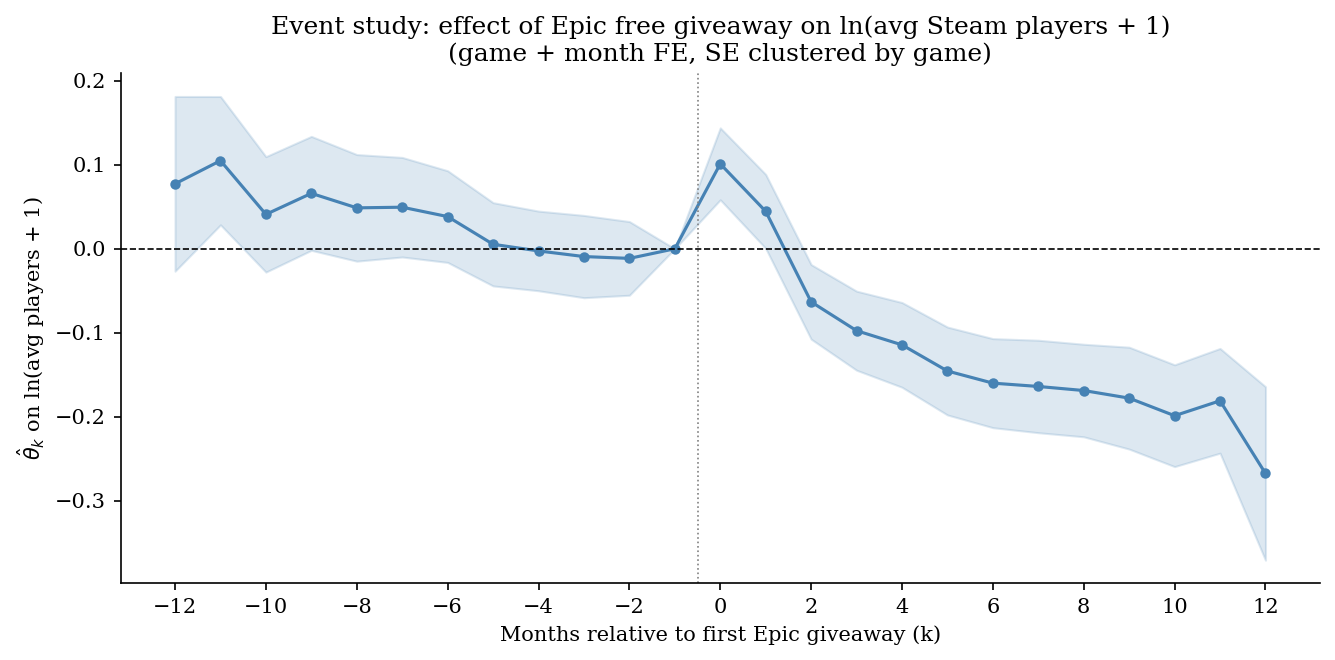
\includegraphics[width=\linewidth]{../output/fig_event_study_pooled.png}

  \vspace{-0.2em}
  {\small Pooled TWFE. Game + calendar-month FE. $N = 38{,}641$; 446 games. Reference: $k=-1$.}

\column{0.43\textwidth}
  \textbf{Phase 1 --- Advertising spike}
  \begin{itemize}
    \item $k=0$: \alert{$\hat\theta_0 = +0.101$} $(p<0.001)$ $\Rightarrow$ $\approx$\alert{10.6\%} more Steam players
    \item Consistent across all estimators: \alert{+5 to +14\%} at $k=0$
    \item Placebo $p < 0.001$; actual estimate is 2.7$\times$ the 95th percentile of null
  \end{itemize}

  \vspace{0.5em}
  \textbf{Phase 2 --- Substitution reversal}
  \begin{itemize}
    \item Turns negative by $k=2$ ($-6.3\%$, $p=0.005$)
    \item \alert{$-10$ to $-23\%$} below baseline by $k=12$ across estimators
    \item Significant at 5\% under all three robust estimators from $k=5$ onward
  \end{itemize}

  \vspace{0.4em}
  \textbf{Repeat giveaways:} $\hat\delta = 0.0001$ $(p = 0.999)$ --- zero additional effect
\end{columns}

\end{frame}

% ── SLIDE 5: ESTIMATOR COMPARISON (OPTIONAL / can skip for time) ──────────────
\begin{frame}{Robustness: All Four Estimators Agree}

\begin{columns}[T]
\column{0.55\textwidth}
  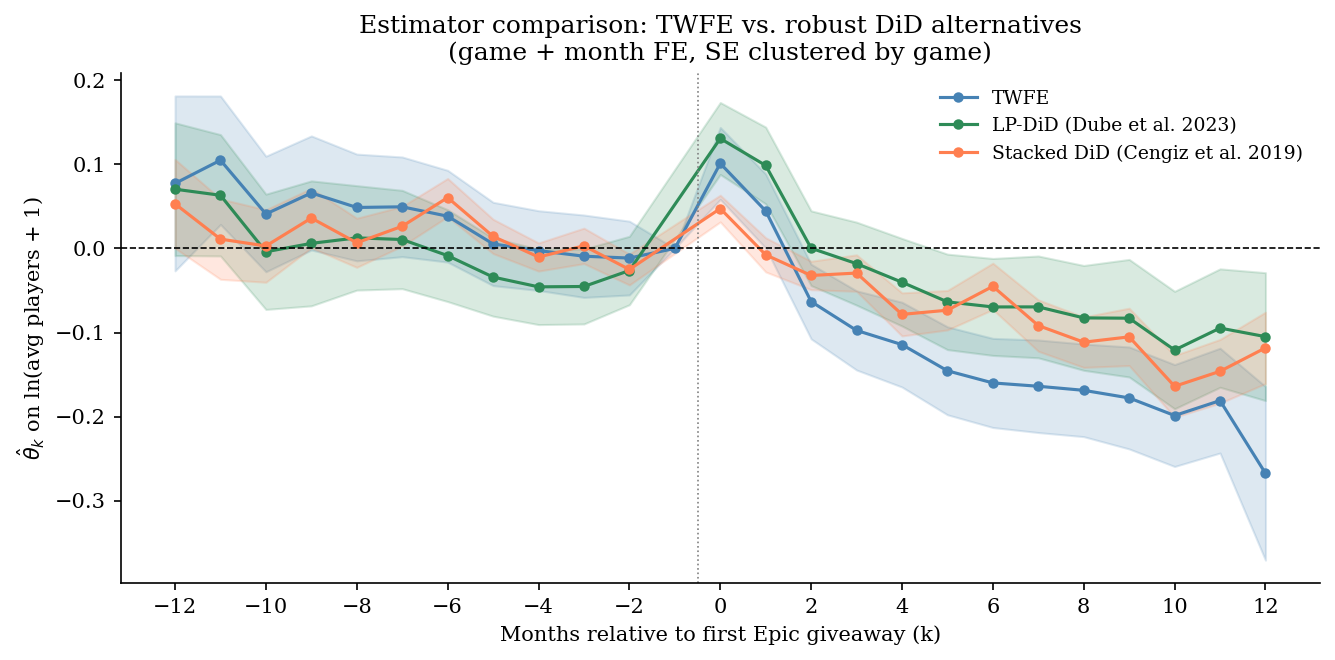
\includegraphics[width=\linewidth]{../output/fig_estimator_comparison.png}

  {\small TWFE, LP-DiD (Dub\'e et al., 2023), Stacked DiD (Cengiz et al., 2019). Reference: $k=-1$.}

\column{0.43\textwidth}
  \vspace{0.3em}

  \begin{tabular}{lccc}
    \toprule
    $k$ & TWFE & LP-DiD & Stacked \\
    \midrule
    $0$  & $+0.101^{***}$ & $+0.131^{***}$ & $+0.047^{***}$ \\
    $1$  & $+0.045^{*}$  & $+0.099^{***}$ & $-0.008$ \\
    $2$  & $-0.063^{**}$ & $\phantom{+}0.000$ & $-0.032^{***}$ \\
    $5$  & $-0.145^{***}$ & $-0.064^{*}$ & $-0.073^{***}$ \\
    $10$ & $-0.199^{***}$ & $-0.121^{***}$ & $-0.164^{***}$ \\
    $12$ & $-0.267^{***}$ & $-0.105^{**}$ & $-0.118^{***}$ \\
    \bottomrule
  \end{tabular}

  \vspace{0.5em}
  \textit{\small $^*p<0.05$, $^{**}p<0.01$, $^{***}p<0.001$. SE clustered by game.}

  \vspace{0.4em}
  All estimators agree: \alert{short-run positive spike, sustained medium-run reversal}. Spread at $k=0$ (0.047 to 0.131) bounds the true ATT.
\end{columns}

\end{frame}

% ── SLIDE 6: TAKEAWAYS & CAVEATS ─────────────────────────────────────────────
\begin{frame}{Takeaways, Caveats \& Future Work}

\begin{columns}[T]
\column{0.50\textwidth}
  \textbf{Main takeaway}

  Both mechanisms are correct --- at different horizons:
  \begin{itemize}
    \item \textbf{Short run:} Giveaway announcement $\rightarrow$ media coverage $\rightarrow$ Steam awareness spike (\alert{+5--14\%})
    \item \textbf{Medium run:} Free Epic copy gradually substitutes Steam engagement (\alert{$-$10--23\%} by month 12)
    \item Epic's free-game program may inadvertently function as \alert{Steam advertising}
  \end{itemize}

  \vspace{0.4em}
  \textbf{Implications}
  \begin{itemize}
    \item For developers: net benefit depends on Epic payment vs.\ long-run Steam erosion
    \item Repeat giveaways add no marginal value ($\hat\delta \approx 0$)
  \end{itemize}

\column{0.47\textwidth}
  \textbf{Caveats}
  \begin{itemize}
    \item \textbf{No never-treated group} --- identification rests entirely on timing variation; parallel trends untestable in absolute sense
    \item \textbf{Player counts $\neq$ purchases or revenue} --- SteamCharts measures concurrent players, not sales
    \item \textbf{Genre heterogeneity} --- single-player vs.\ multiplayer titles have different substitution dynamics (pooled estimate conflates them)
    \item \textbf{DLC/bundle events} --- 15 giveaways were DLC mapped to base-game Steam IDs
  \end{itemize}

  \vspace{0.4em}
  \textbf{Future work}
  \begin{itemize}
    \item Genre-stratified analysis (single-player vs.\ multiplayer)
    \item Study effects on Steam \emph{sales} volume
    \item EGS-side engagement data (currently unavailable)
  \end{itemize}
\end{columns}

\end{frame}

% ─────────────────────────────────────────────────────────────────────────────
% Citations used inline throughout slides; no bibliography slide needed.

\end{document}
